\section{Descrição do cenário} \label{sec:cenario}
Para o desenvolvimento da pesquisa, deve-se definir um cenário em que as aplicações das técnicas estudadas nesse trabalho sejam viáveis. Logo, o cenário definido deve ser um problema modelado por teoria de filas, tornando possível a aplicação das regras de \textit{clearing function}. Da mesma maneira, o cenário deve ser um problema de produção em lotes com estações de trabalho de processamento em série, podendo aplicar então as técnicas de \textit{lot streaming}.

O problema então conterá um sistema de apenas duas máquinas, de forma a generalizar, uma vez que um problema de $m$ máquinas pode ser resolvido como $m-1$ subproblemas de duas máquinas, ou seja, dominar a resolução do problema de duas máquinas garante que pode ser resolvido um caso mais geral de 3, 4,\ldots, $m$ máquinas \cite{Potts1989,Trietsch1993,Baker1995}.

Além disso, o tamanho do lote de produção do problema inicial deve ser suficientemente grande para divisão em sublotes menores, de modo que os sublotes possam ser processados em paralelo nas estações de trabalho (\textit{overlapping}), tornando possível a diminuição do tempo de completude das atividades (\textit{makespan}).

\citeonline{Trietsch1993} apresentam um exemplo de cenário em que o \textit{lot streaming} é aplicado e resolvido de diferentes maneiras. Considerando um exemplo contendo um lote de 84 itens a serem processados em três máquinas, sendo a máquina 1, 2 e 3, com tempos de processamento de 2, 1 e 3 minutos por item, respectivamente. Sem a divisão do lote, ou seja, sem o uso do \textit{lot streaming}, o \textit{makespan} é de 504 minutos. 

Em um primeiro caso onde considera-se dois sublotes iguais e sem ociosidade entre máquinas, chega-se ao \textit{makespan} de 420 minutos, redução de 16,7\%, conforme mostrado na Figura~\ref{fig:LS_ex1}. Uma segunda situação, Figura~\ref{fig:LS_ex2}, onde continua-se com dois sublotes iguais, porém permitindo a ociosidade intermitente, o \textit{makespan} é reduzido para 378 minutos, melhoria de 25\%. Já na Figura~\ref{fig:LS_ex3}, é permitido que os lotes sejam variados entre os pares de máquinas, reduzindo o \textit{makespan} para 385, representando uma redução de 23,6\%. Por fim, permitindo a variabilidade dos sublotes e ociosidade intermitente, obtêm-se o tempo total de 360 minutos, redução de 28,6\%, Figura~\ref{fig:LS_ex4}. Ainda, os autores destacam que neste último em particular os sublotes se mantiveram consistentes no decorrer do sistema, diferentemente do problema da Figura~\ref{fig:LS_ex3}, ao qual eles variaram.

\begin{figure}[!ht]
    \centering
    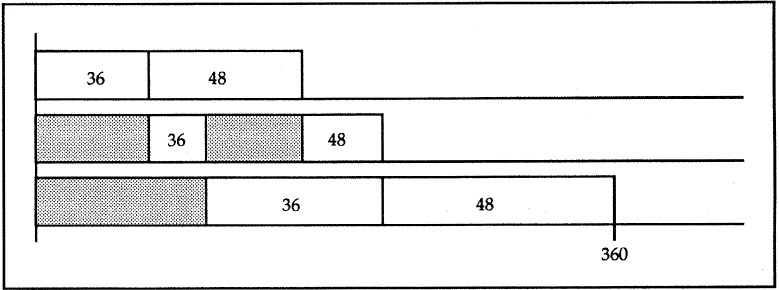
\includegraphics[scale=0.4]{Referencial/Figuras/Ls_ex4}
    \caption{Solução para o exemplo com dois lotes iguais e sem ociosidade}
    \label{fig:LS_ex1}
\end{figure}

\begin{figure}[!ht]
    \centering
    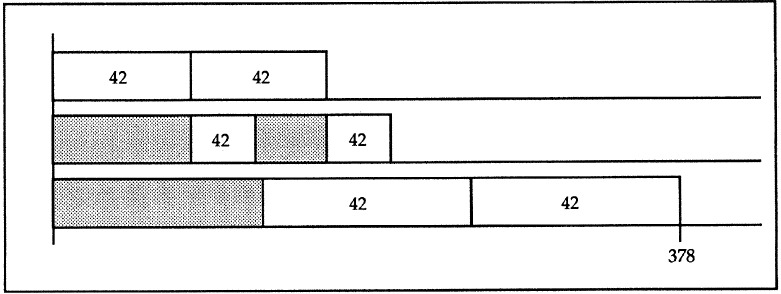
\includegraphics[scale=0.4]{Referencial/Figuras/Ls_ex2}
    \caption{Solução para o exemplo com dois lotes iguais e ociosidade intermitente}
    \label{fig:LS_ex2}
\end{figure}

\begin{figure}[!ht]
    \centering
    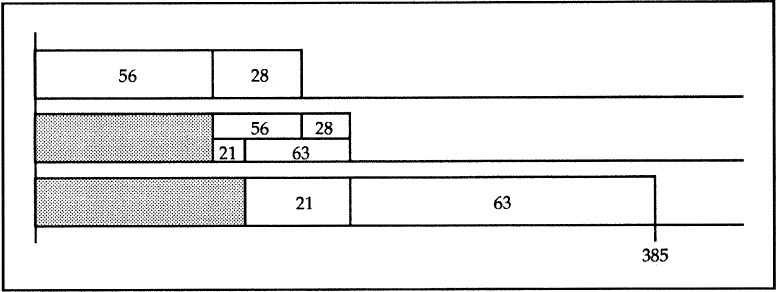
\includegraphics[scale=0.4]{Referencial/Figuras/Ls_ex3}
    \caption{Solução para o exemplo com dois lotes variáveis e sem ociosidade}
    \label{fig:LS_ex3}
\end{figure}

\begin{figure}[!ht]
    \centering
    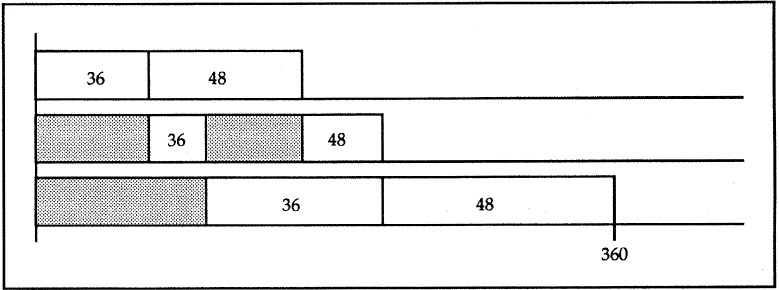
\includegraphics[scale=0.4]{Referencial/Figuras/Ls_ex4}
    \caption{Solução para o exemplo com dois lotes variáveis e ociosidade intermitente}
    \label{fig:LS_ex4}
\end{figure}